\documentclass[11ptm,oneside,a4paper]{report}

\usepackage{booktabs}
\usepackage[utf8]{inputenc}
\usepackage[scale=2]{ccicons}
\usepackage{subcaption}
\usepackage{float}
\usepackage{amsmath}

\usepackage{tikz}
\usetikzlibrary{positioning}

\usepackage{pgfplots}
\usepgfplotslibrary{dateplot}
\usepackage{amsthm,amsmath,amsfonts,amssymb,listings,titling,graphicx,epsfig,epstopdf,url,array}
\usepackage{verbatim}
\usepackage{pdfpages}
\usepackage[nottoc]{tocbibind}
\usepackage{xspace}
\newcommand{\themename}{\textbf{\textsc{metropolis}}\xspace}

\definecolor{chromeyellow}{rgb}{1.0, 0.65, 0.0}
\definecolor{chocolate(web)}{rgb}{0.82, 0.41, 0.12}
\definecolor{cornflowerblue}{rgb}{0.39, 0.58, 0.93}
\definecolor{flame}{rgb}{0.89, 0.35, 0.13}
\definecolor{coquelicot}{rgb}{1.0, 0.22, 0.0}
\definecolor{darkspringgreen}{rgb}{0.09, 0.45, 0.27}

\usepackage{graphicx}
\usepackage{amssymb}
\usepackage{lineno}

\def\be{\begin{equation}}
\def\ee{\end{equation}}
\def\pa{\partial}
\newcommand{\HRule}{\rule{\linewidth}{0.5mm}}


\begin{document}

\vspace*{\stretch{1.0}}
\begin{center}
\Large\textbf{Modelling of the diffusion inside a dialysis button - 
Application to the Crystallisation of membrane proteins} \\
% \large\textit{Virginia Apostolopoulou}
\end{center}
\vspace*{\stretch{2.0}}


%% Title, authors and addresses

\section{Introduction}

Protein crystallization is a complicated physico-chemical process: a specific macromolecule often crystallizes in a narrow range of several parameters, including concentration, temperature, pH, nature and concentration of crystallization agent, presence of counter-ions, impurities, and other chemical additives, as well as method and rate of supersaturation generation. This means that different methods of crystallizing the same protein may give rise to different quantities and qualities of crystals even under the same state of the mother liquor (A. McPherson, 1999, Crystallization of Biological Macromolecules, Cold Spring Harbor Laboratory Press, Cold Spring Harbor) 
In dialysis, considered as the first membrane operation used to perform crystallization, diffusion and equilibration of precipitant molecules through semipermeable membrane is used to slowly approach the concentration at which the macromolecule crystallizes by salting-out effect (Zeelen J.P. Wierenga R.K., 1992, J. Cryst. Growth. 122, 194-198). The transfer of solutes and solvent through semipermeable membranes provides the slowly varying conditions required for early crystal nucleation and relatively undisturbed lattice formation of crystal growth (Zeppezauer M., Eklund E., Zeppezauer E., Arch. Biochem. Biophys., 1968, 126, 564-573;  Madjid A.H., Vaala A.R., Pedulla Jr. J., et al., 1972, Phys. Status Solidi, 12, 575-579.) Since then, several other membrane operations, such as reverse osmosis, membrane distillation, osmotic distillation, forward osmosis, etc… are used to realize membrane-assisted crystallization. 
Membrane-assisted crystallization technology is at the basis of the crystallization apparatus developed recently with the focus to monitor and control the crystallization processes in situ generating the crystals of specific sizes and morphology optimized for different downstream structure determination approaches (Junius et al., J. Applied Cryst. 2016). 
Nucleation and crystal growth are supersaturation-dependent. Usually, low supersaturation favors crystal growth while higher values are associated with excessive nucleation. The consequence of the supersaturation degree in a crystallization trial is the relative extent of the nucleation over the crystal growth rate, while the macroscopic evidence is on crystal morphology and size.  
In membrane-assisted crystallization, the membrane acts as a dosing device to generate supersaturation. Mass transfer, quantified in terms of transmembrane flux, is fixed by the proper combination of the operational parameters and membrane properties, which affect the specific driving force. As mentioned, in protein crystallization the macromolecule, precipitant agent, buffer, and potential additives, compose the crystallizing solutions. Several parameters like solute, precipitant, and draw solution concentration, have influence on the flux by acting on the partial pressure of the solvent (water) in the crystallizing solution. Generally, increased concentration of components in solution is associated to a reduced driving force for solvent evaporation. Additionally, as crystallizing solution concentration increases because of solvent evaporation, the driving force decreases even more, thus reducing the rate of solution concentration (transmembrane flux). To maintain a constant transmembrane flux and supersaturation rate, changes in solution composition because of solvent removal can be counterbalanced by corrections in the driving force by acting on operative temperature and stripping solution concentration. These parameters can be controlled in time during the crystallization as the macromolecular solution increases its concentration, so that the state of the system moves along a well-defined trajectory in the phase diagram. Therefore, the extent of the crystalline population, the morphological (size, habit, and shape) and structural (polymorphism) crystal properties can be controlled. 
  
The concept of membrane crystallization combines the principles of mass (and heat) transport through porous membranes and the theory of heterogeneous nucleation occurring at the interface with polymeric films. In addition, morphological parameters such as porosity or roughness, as well as the hydrophobic character of the membrane (expressed in term of contact angle, surface tension, etc.) significantly affect the crystallization kinetics. All these aspects are quantitatively related to each other; the intensity of transmembrane flux affects the rate of supersaturation generation and, consequently, the nucleation rate. Moreover, the classical nucleation theory adapted to the case of microporous membranes clearly defines the mathematical relationship existing between the physico-chemical properties of polymeric surface and the nucleation kinetics. 
 
This article aims to provide a simple predictive model of mass transport explaining the crystallization process and eventually the nucleation phenomena observed experimentally with the recently developed instrument. 
Our interest in combining membrane operations, solution crystallization and modeling is motivated by the aim to develop more efficient crystallization processes in the field of biological crystallization. We aim to use the membrane as precision device to control the composition of the crystallizing solution, the level of supersaturation and its generation rate by tuning the mass transfer across the membrane… 

\section{How did the work}

\section{Materials and Methods} \label{methods}

\subsection{Experimental set-up}

The experiment is based on the crystallisation apparatus for temperature-controlled flow-cell dialysis
\cite{Junius:ei5002}. The principle of this method is the diffusion of a small molecules through a semi-permeable membrane. 
In order to optimize such devices, but also to understand the underlying processes, such as the equilibrium concentration times of the crystallisation agents between the reservoir and the dialysis chamber, 
a systematic study of the diffusion kinetics was contacted. 
More precisely, we focus on the diffusion of the crystallisation agents through the dialysis membrane. 
The membrane separating the dialysis chamber from the reservoir limits the diffusion of the molecules from the
reservoir to the crystallisation chamber. The semi-permeable membrane used in the experiment is a cellulose membrane, persuaded from Spectrum Labs. It can be described by its molecular weight cutoff (MWCO), i.e. its pore size measured in angstrom units. A larger MWCO corresponds to a wider pore size. The membrane in the experiment is chosen such as the protein cannot diffuse across the crystallisation chamber. 

Measurements were made of the characteristic diffusion times for different families of crystallisation agents. 
We used two families of agents, commonly used in crystallisation of proteins: 
polyethene glycol (PEG) and salts. The molecular weight (MW)
of PEG was varied between 1000 and 8000. Measurements of three different salts were made: 
sodium chloride (NaCl), sodium acetate (NaOAc) and ammonium sulphate ((NH$_4$)$_2$S0$_4$).  

We use the dialysis button described in \cite{Junius:ei5002}, but instead of protein solution, it contained distilled water. The 
button is covered with a standard RC membrane Spectra/Por (https://www.spectrumlabs.com) with a molecular cutoff 
of either $12-14$ kDa or $3.5$ kDa. 
Each button is placed individually inside a reservoir containing the crystallisation agent we wish to study.
The experiment is carried out at two different temperatures in order to study the effect of temperature on the diffusion.
The reservoir is kept to a constant temperature of $277$ K and $293$ K, respectively. The button is placed inside the reservoir of 
constant temperature. After a given time, i.e. 30 min, 1 h, 2 h, etc., 
then the dialysis button is recovered with a tweezer and the dialysis membrane is removed \ref{set_up}. 
Then the dialysis chamber is mixed using a pipette and a volume of at least 30 $\mu$L is taken. 
The sample is then placed on the surface of the prism of the refractometer in order to measure the refractive index of the solution. 
The refractometer that is used is the Carl Zeiss with a precision of $\pm 0.001$ on the refraction index.

\begin{figure}[H]
  \begin{center}
      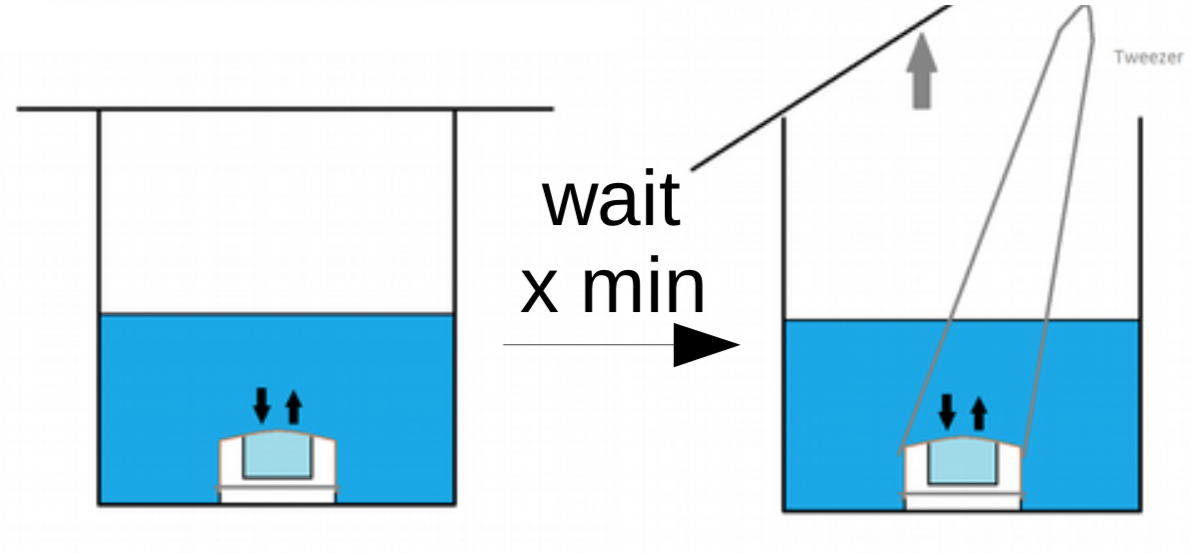
\includegraphics[scale=0.33]{figures/set_up.png}
      \caption{Schematic representation of steps followed to get the concentration 
      meassurments for a specific time. }  
      \label{set_up}
  \end{center} 
\end{figure}
\noindent

To establish the relationship between the refractive index and the concentration of each solution we established the calibration curve. 
The refractive index is a dimensionless number that depends on several variables, 
such as temperature, concentration, wavelength and more, i.e  
$n = f(T, [C], \lambda, \dots)$. For all the measurements white light is used.
To reduce the scattering effect due to the use of polychromatic source, 
a scroll wheel is located on the refractometer to help with the adjustment of several prisms of different glasses in the path of the beam. All the measurements were made at ambient pressure. 


The measurements of the concentration of the two compounds that diffuse through a membrane 
can be used to estimate the permeability coefficient of the membrane, defined as 
$P_m = \frac{N}{A_m \Delta S}$ with units cm/h, and eventually calculate the permeability rate, which is impossible to measure precisely in an experiment. 
The permeability coefficient can be estimated by measuring the 
\textit{half-escape time}, 
i.e. the time in which the concentration in the dialysis button reaches half of the initial concentration of the reservoir \cite{pmid4889148}. Using the concentration measurements through time obtained from the experiment, we can use an
exponential fitting to estimate the half-escape time for our system. For the fitting we used the following formula:

\be
  y(x) = 1 - e^{-ct}, 
\ee
where $c$ is a paramater evaluated using a non-linear least squares function. 

Figure \ref{exp-peg1000} and
\ref{exp-salt} show the concentration  as a function of time for PEG 1000 at $5\%$ (w/v) and NaCl at $0.5$ molL$^{-1}$, respectively. The points correspond to the experimental measurements and the line corresponds to the exponential fitting. We calculated the half-escape time for the case of PEG 1000, $0.5\%$ (w/v) to be $5.19$ h and for the case of NaCl, $2$ molL$^{-1}$ to be $42$ min. We can see that the behaviour of the two crystallisation agents is different and that NaCl diffuse faster than the PEG.

\begin{figure}[t]
  \begin{center}
  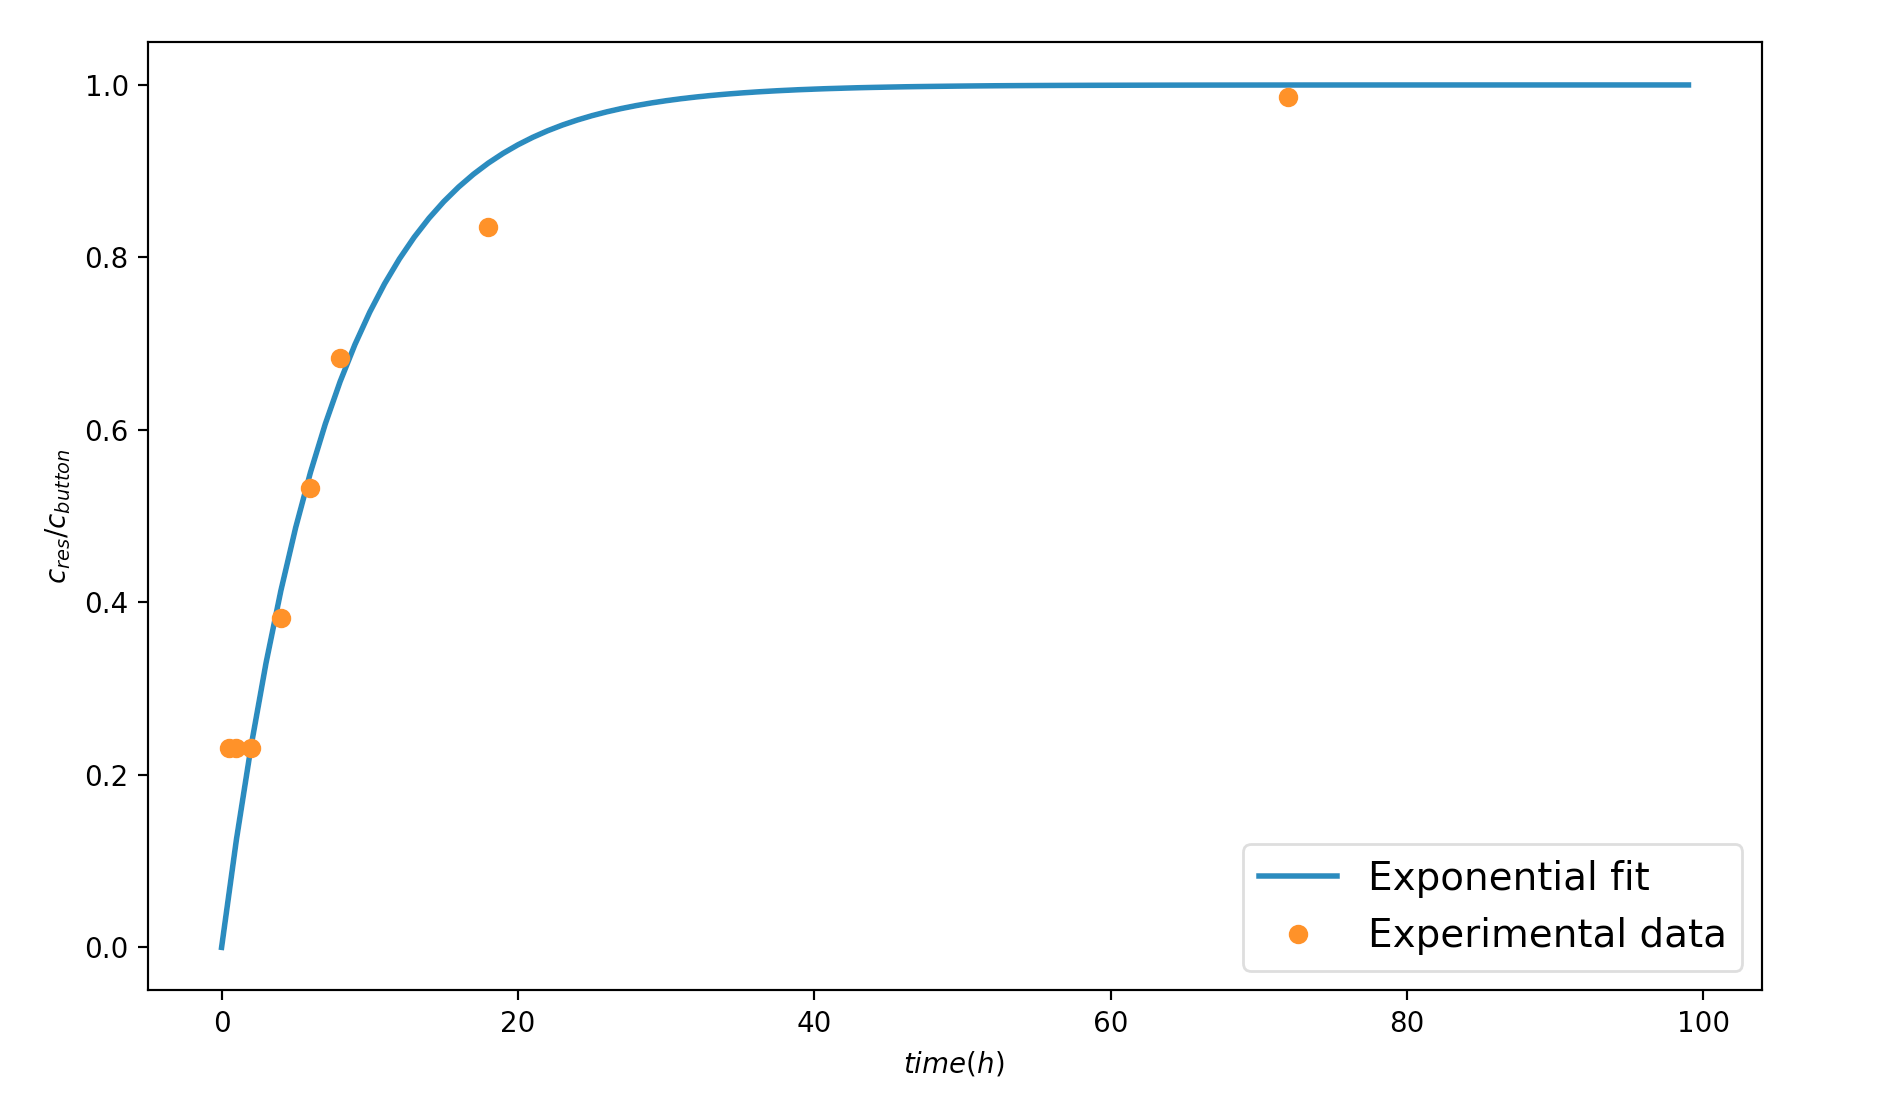
\includegraphics[scale=0.25]{figures/exponentional_fit_PEG1000.png}
      \caption{Evolution of the concentration of PEG 1000 as a funcion of time. The $t_{1/2}$ was calculate to be around $5.19$ h \label{exp-peg1000}}  
  \end{center} 

\end{figure}
\noindent 

\begin{figure}[t]
  \begin{center}
      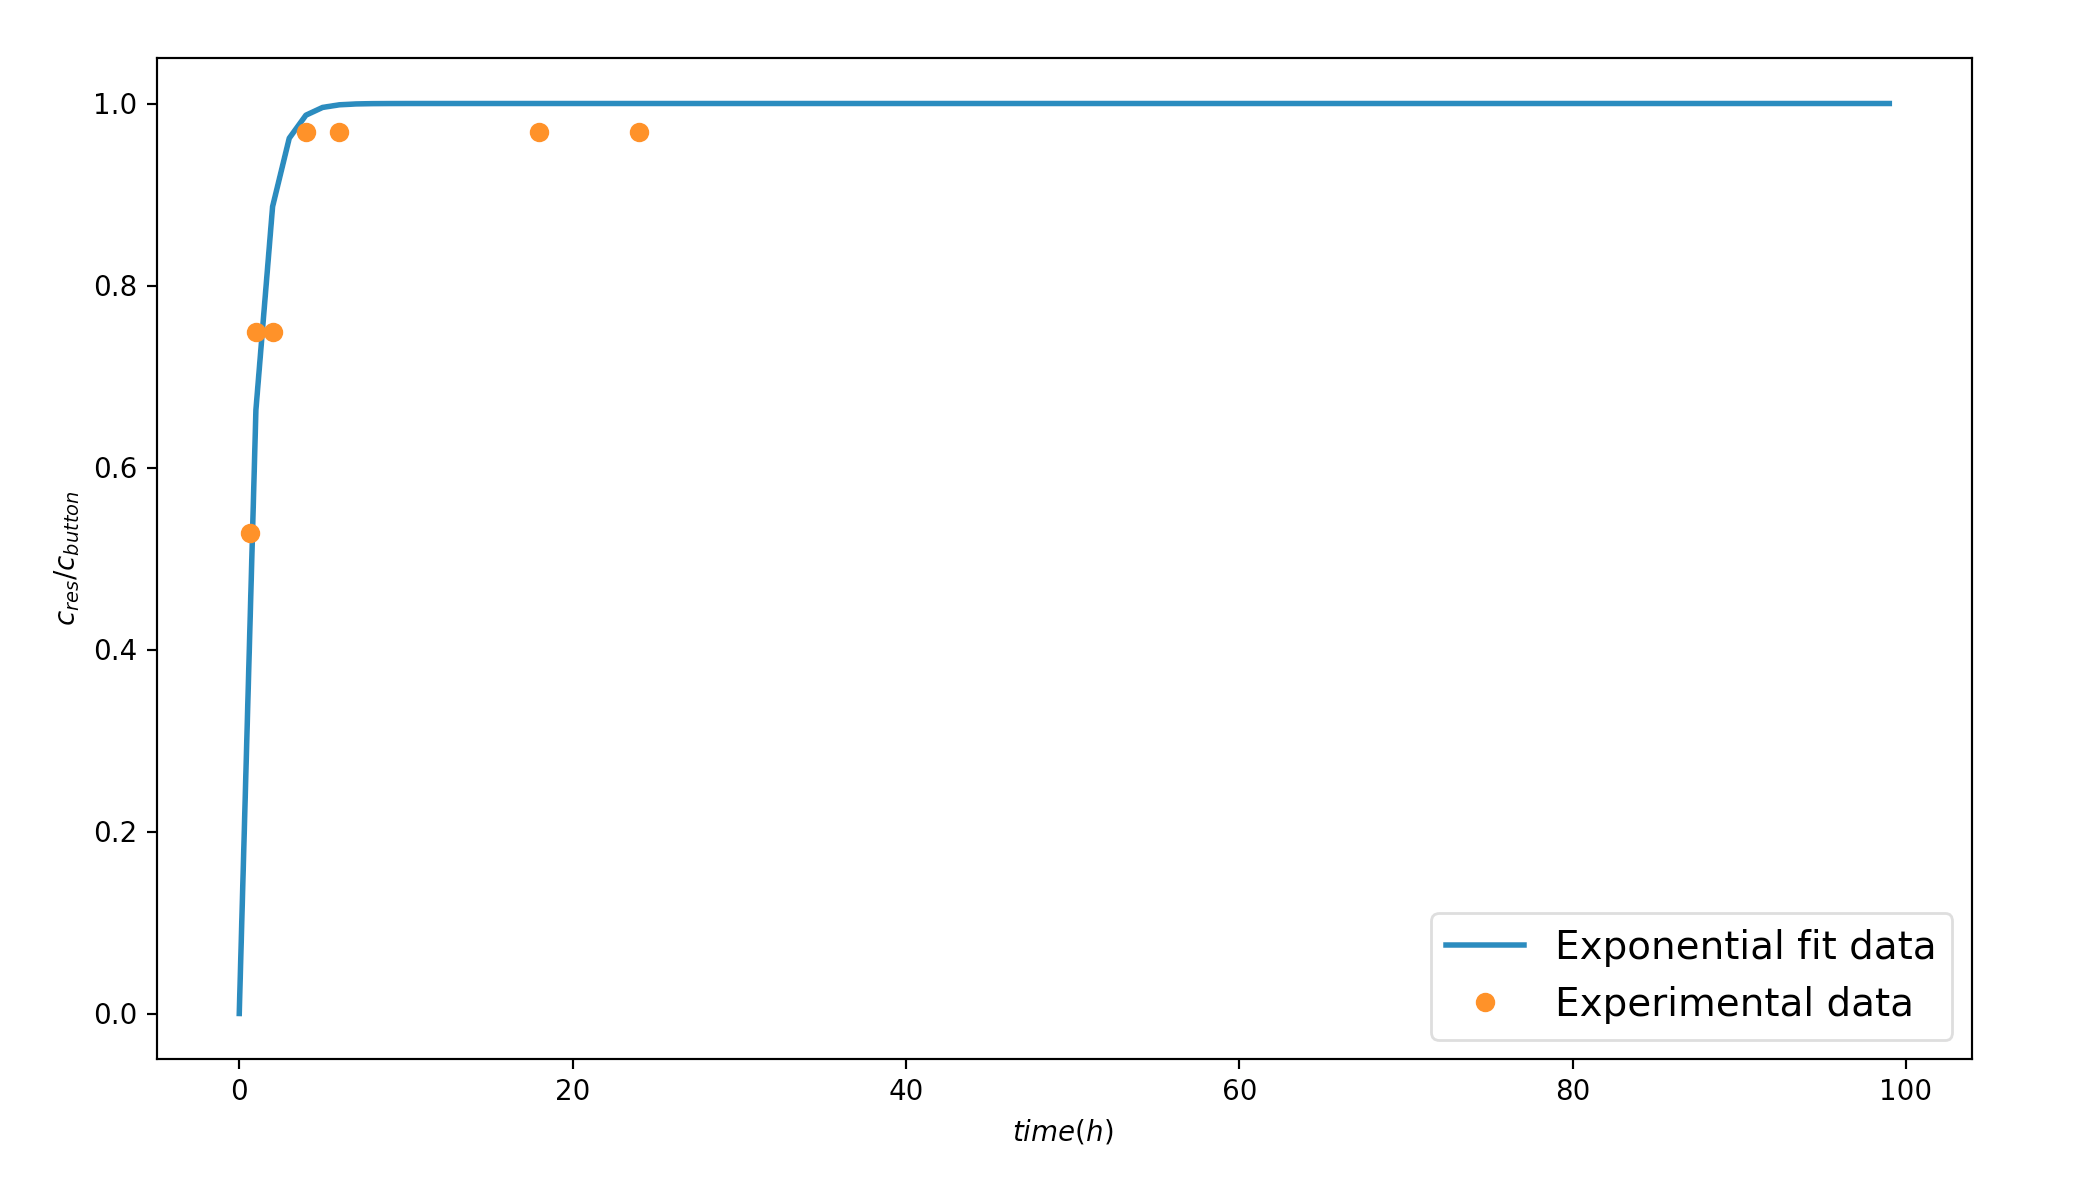
\includegraphics[scale=0.23]{figures/exponentional_fit_SALT.png}
      \caption{Evolution of the concentration of NaCl as a funcion of time. The $t_{1/2}$ was calculate to be around $42$ min  \label{exp-salt}}   
  \end{center} 
\end{figure}

\subsection{The diffusion model}\label{theory}

The experimental diffusion profiles for the crystallisation agents through a crystallisation membrane can be described by a Fickian diffusion model. The features of the model follow.

As discussed, the experimental set-up includes an effectively very large reservoir
with a give concentration of salt or of PEG, separated for the dialysis button by a 
membrane. The diffusion process inside the button using the 
diffusion equation for the $z-axis$ can be described as follows:

\begin{equation}
\frac{dc}{dt} = D \frac{d^2 c}{dz^2}
\end{equation}
where we note $c$ as the concentration of the percipitant in the z-direction and 
$D$ the diffusion coefficient m$^2$ s$^{-1}$.

The diffusion coefficient is a constant for a given percipitannt under a given set of conditions. It depends on the molecular size (here given in molecular weight) and the concentration. 

The flux density $(J)$ across the membrane is given by:

\begin{equation} \label{flux}
    J = P\Delta c = P(c_{res} - c_{button}), 
\end{equation} 
where $c_{res}$, $c_{button}$ is the concentration imposed outside the 
button and the concentration inside the button, respectively, 
and $P$ is the permeability rate (1/h).
Hence, the flux density is equal to the permeability coefficient times the difference in concentration across the membrane. The values of $P$ 
is depending on the system, i.e. 
the membrane and the diffusive molecules. 


\subsection*{P\'{e}clet number}


In order to quantify the competition between
the phenomenon of diffusion across the length L and the flux of the system, we calculate the dimensionless P\'{e}clet number. The 
P\'{e}clet number measures the dominant mechanism in the system, which can 
either be the time needed for the solution to diffuse across the button or 
the time needed to cross the membrane:

\begin{equation}
    \mathcal{P }e = \frac{L^2/D}{(1/P)} = \frac{L^2 P}{D},
\end{equation} 

where: $L$ is the characteristic length scale, $D$ is the characteristic diffusion coefficient. and $P$ is the permeability rate. In the calculations we used the height of the button, i.e. $L = 5$ $\mu$L.  


We can see that the P\'{e}clet number is proportional to the system size. This means that it depends on the distance over which transport is happening. 
When the P\'{e}clet number is greater than one, the permeability effect exceeds the diffusion effect in determining the overall mass flux. 


\section{Results and Analysis}

\subsection{Experimental Results}

\subsection*{Concentration}

The effect of concentration on the variation of diffusion times was studied for PEG 1000, 
4000, 6000, and 8000, at different concentrations, from $5$\% to $30$\%. Figure 
\ref{niels_peg_conc} shows the values of half-escape time $\tau_{1/2}$ obtained 
for the PEG in concentration from $10$\% to $30$\% (NOTE: This was done because Niels
didn't want to put too much info in the graph. In my bar graph, I can include the $5$\% values 
since these are the ones that I had modeled). The membrane used in these experiments had a 
retention threshold of $12-14$ kDa, with constant temperature of $293$ K. The volume of the
dialysis chamber is $200$ $\mu$L. When the concentration of PEG increases. the value of 
$\tau_{1/2}$ decreases. On the other hand, the increase of the molecular weight of PEG shows
an analogous increase of $\tau_{1/2}$. These results are coherent with the fact that at a
given pore size the larger molecules will diffuse slower than the smaller molecules.
 
\begin{figure}[!htb]
  \begin{center}
      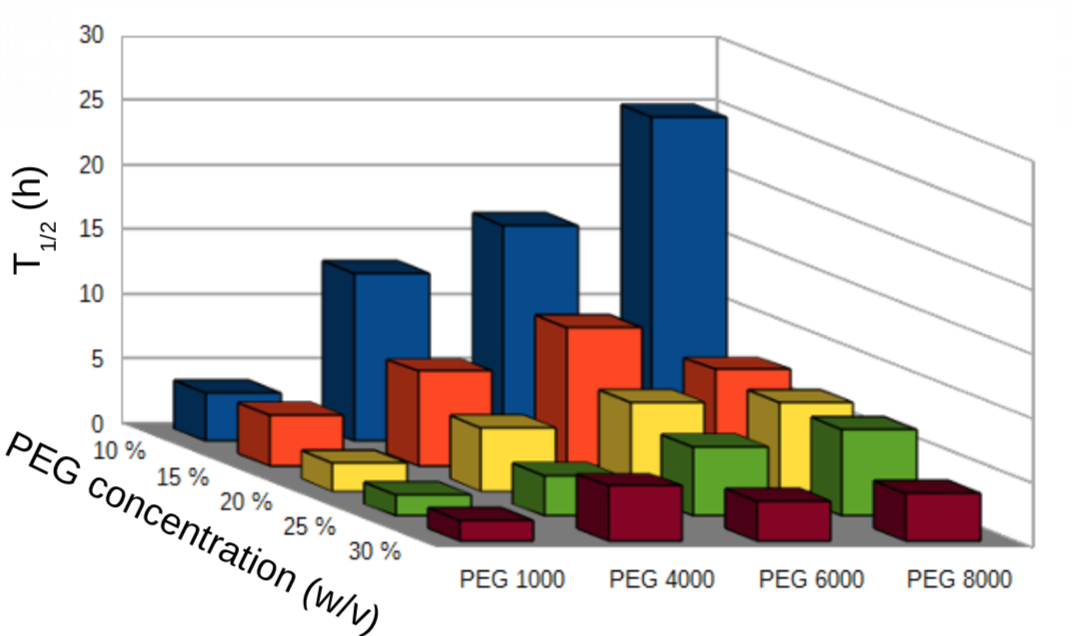
\includegraphics[scale=0.4]{figures/Niels-PEG-conc.png}
      \caption{\label{niels_peg_conc}}  
  \end{center} 
\end{figure}
\noindent
This values indicate that an experiment for PEG 1000 will reach the desired supersaturation in 
the dialysis chamber in a few hours in the case of concentrations larger than $15$\% for a 
membrane of MWCO $12-14$ kDa, in constant temperature of $293$ K. For PEG 4000 to 8000 
$\tau_{1/2}$ is much higher for concentration larger than $15$\%. 

The respective results for the salts are shown in Figure \ref{niels_salt_conc}. The salts diffuse much faster compared to PEG. Regardless of the initial concentration of the salt
from $0.5$ to $3$ molL$^{-1}$, $\tau_{1/2}$ will be in order of $60$ min or lower. 
As for the effects of concentration and molecular weight, one can observe the same trends 
as in the case of PEG.

\begin{figure}[!htb]
  \begin{center}
      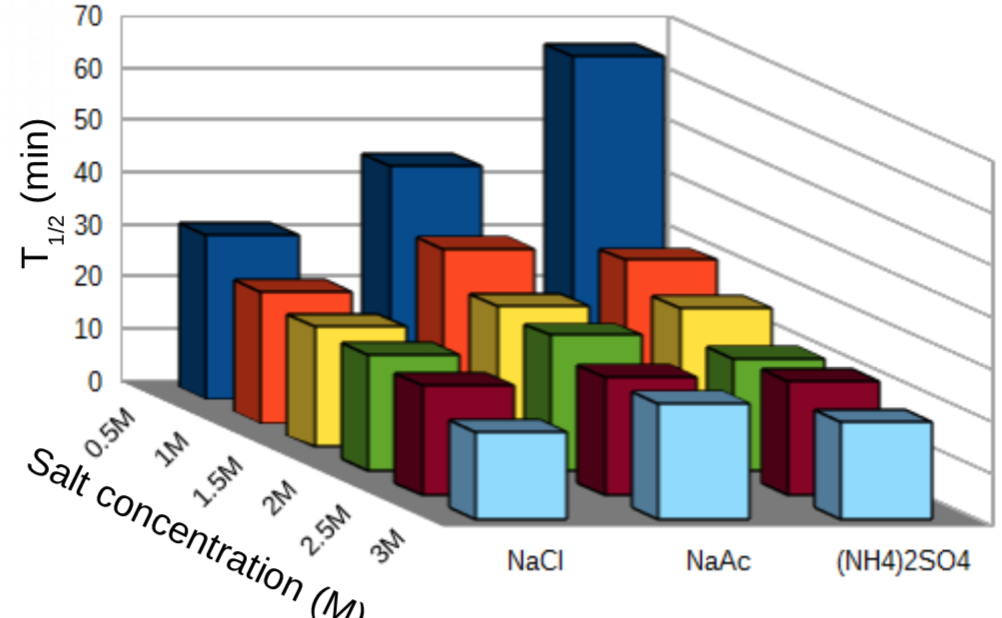
\includegraphics[scale=0.4]{figures/Niels-placeholder-SALTS-concentrations.png}
      \caption{\label{niels_salt_conc}}  
  \end{center} 
\end{figure}

\subsection*{Temperature}

The effect of the temperature on diffusion 
was studied by performing the same experiment for two different 
temperatures; $277$ K and $293$ K. As is shown in Figures \ref{niels_temp_peg} and 
\ref{niels_temp_peg8000} there is a small effect of temperature in the diffusion of 
PEG 1000, which becomes larger as the molecular weight of PEG increase. 
 
\begin{figure}[!htb]
  \begin{center}
      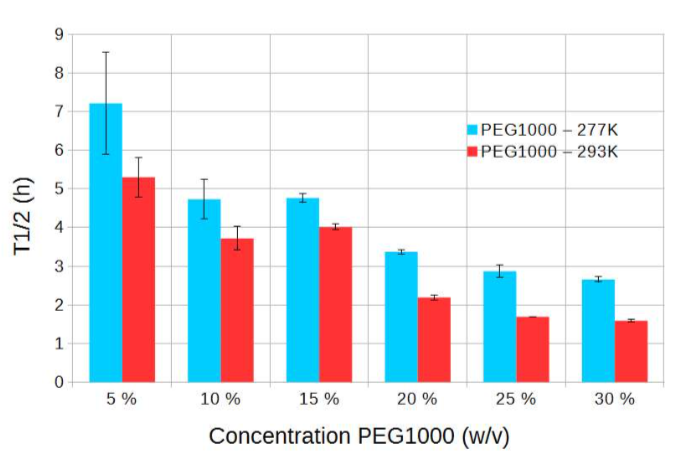
\includegraphics[scale=0.5]{figures/Niels-temperature-PEG1000.png}
      \caption{\label{niels_temp_peg}}  
  \end{center} 
\end{figure}

\begin{figure}[!htb]
  \begin{center}
      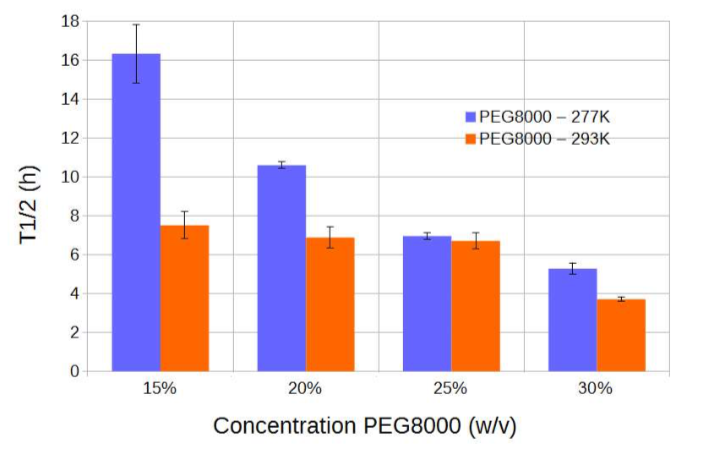
\includegraphics[scale=0.5]{figures/Niels-temperature-PEG8000.png}
      \caption{\label{niels_temp_peg8000}}  
  \end{center} 
\end{figure}
\noindent
The effect of the temperature on the values of $\tau_{1/2}$ is expected, since 
the diffusion coefficient has a dependence on the temprerature. According to the 
Stokes-Einstein equation for spheres in viscous media, the diffusion coefficient is expected to increase as the temperature increases.

\subsection*{Membrane}

Different dialysis membrane was used to study the effect of the pore size threshold of the
membrane. Two dialysis membrane was studied; one of MWCO of $3.5$ kDa and the other of 
$12-14$ kDa. Figure \ref{Niels_membrane} shows the values of $\tau_{1/2}$ for PEG 1000 
and PEG 4000. For PEG 4000, a shift of $2$ to $4$ h on the values of $\tau_{1/2}$ is observed
between the two membranes that were tested. The same trend can be observed in the case of 
PEG 1000.

\begin{figure}[!htb]
  \begin{center}
      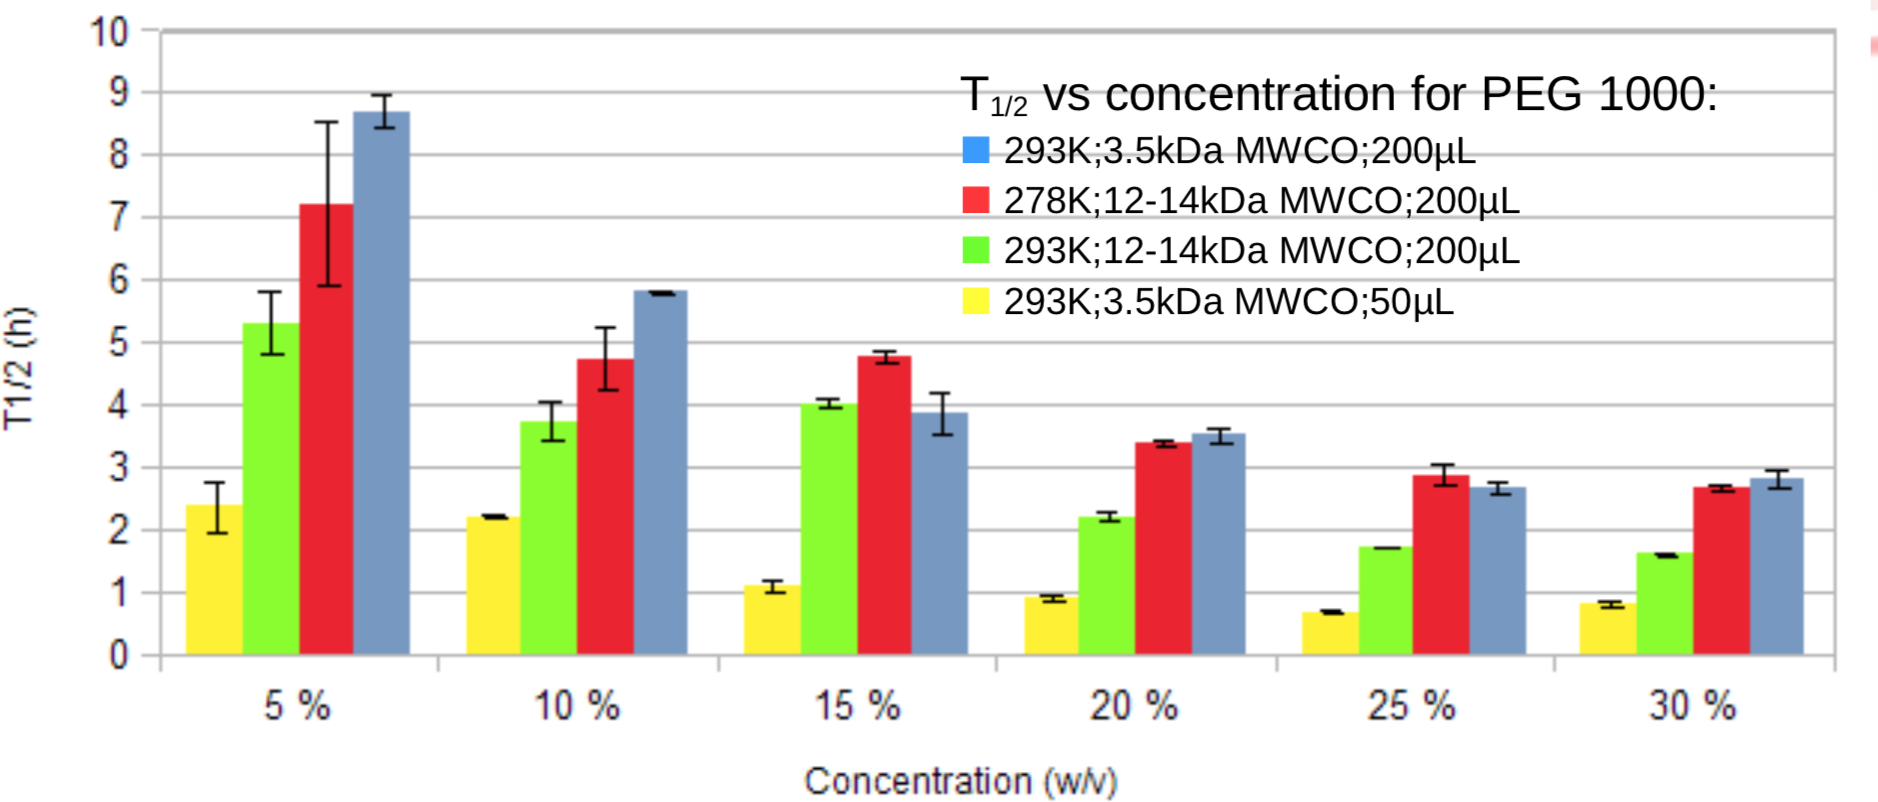
\includegraphics[scale=0.25]{figures/Niels-placeholder-time-PEG1000-membranes.png}
      \caption{\label{Niels_membrane}}  
  \end{center} 
\end{figure}


\subsection{Diffusion model}
    
    As noted in section \ref{methods}, a Fickian model can be used to describe the diffusion through a semi-permeable membrane. The diffusion coefficients used in the simulations were taken from the literature and they can be seen in Table \ref{diffusion_coeff}. 

    \begin{table}[h!]
          \begin{center}
            \caption{Diffusion Coefficients values and sources \label{diffusion_coeff}}
            \label{tab:table1}
            \begin{tabular}{l|r} % <-- Alignments: 1st column left, 2nd middle and 3rd right, with vertical lines in between
              \textbf{Percipitant} & \textbf{D $(m^2s^{-1})$} \\
              % $\alpha$ & {}$\beta$ & $\gamma$ \\
              \hline
              PEG 1000 & $2.7 \times 10^{-10}  $  \ref{LEE20081590}, 
              \ref{LEE20081590} \\
              NaCl & $16 \times 10^{-10} $ \ref{doi:10.1021/ja01589a01}, \ref{doi:10.1021/ja01589a011}, \ref{TF9545001048} \\
            \end{tabular}
          \end{center}
    \end{table}

    Our model is limited form the overlapped concentration of PEG. This is due to the fact that polymers change their behaviour in solution as a function of concentration. The character of the interaction of a polymer changes significantly as one goes from the dilute to the semidilute solution. This leads to diffusion coefficient to vary with concentration, and, respectively, the equations presented in Section \ref{theory} cannot describe systems in high concentrations. This was also one of the reasons why we are not yet able to simulate the experimental data for salt and PEG mixtures. The concentration of PEG 6000 used in the experiments was about $15$\% and the 
    overlap concentration of PEG 6000 is measured to be around $11.92$ \% \ref{"Crossover regime for diffusion of nanoparticles in polyethene glycol solution: influence of depletion layer"}, which means the PEG in this mixture is already semidilute and
    diffusion coefficient will depend on the concentration. Another factor that affects the behaviour of PEG is the temperature. 
    This could also be observed from the experimental results reported above. Although low temperatures of $277$ K is common in crystallisation experiments, we could find in the literature diffusion coefficients values of PEG for such low temperatures (to be enhanced after discussion in the meeting). 

    Here, we present simulation results for PEG 1000 and NaCl in concentration 
    $5$\% and $0.5$\% respectively. Even in those low concentrations, we can observe that the process is dominant by the permeability rate rather than the diffusion.  
    By comparing the simulation results to the experimental, we can determinate the permeability rate of the membrane.  


    Figure \ref{conc_prof_PEG1000} and \ref{conc_prof_NaCl} shows the concentration profile of PEG 1000 and NaCl, respectively for 
    different P\'{e}clet numbers. For large permeability rate values, the half-escape time $\tau_{1/2}$ is similar to the best fit values that have been calculated from the experiment. This is an indication that the systems are controlled by the permeability, i.e. the time PEG needs to cross across the membrane. 
    \begin{figure}[!htb]
      \begin{center}
          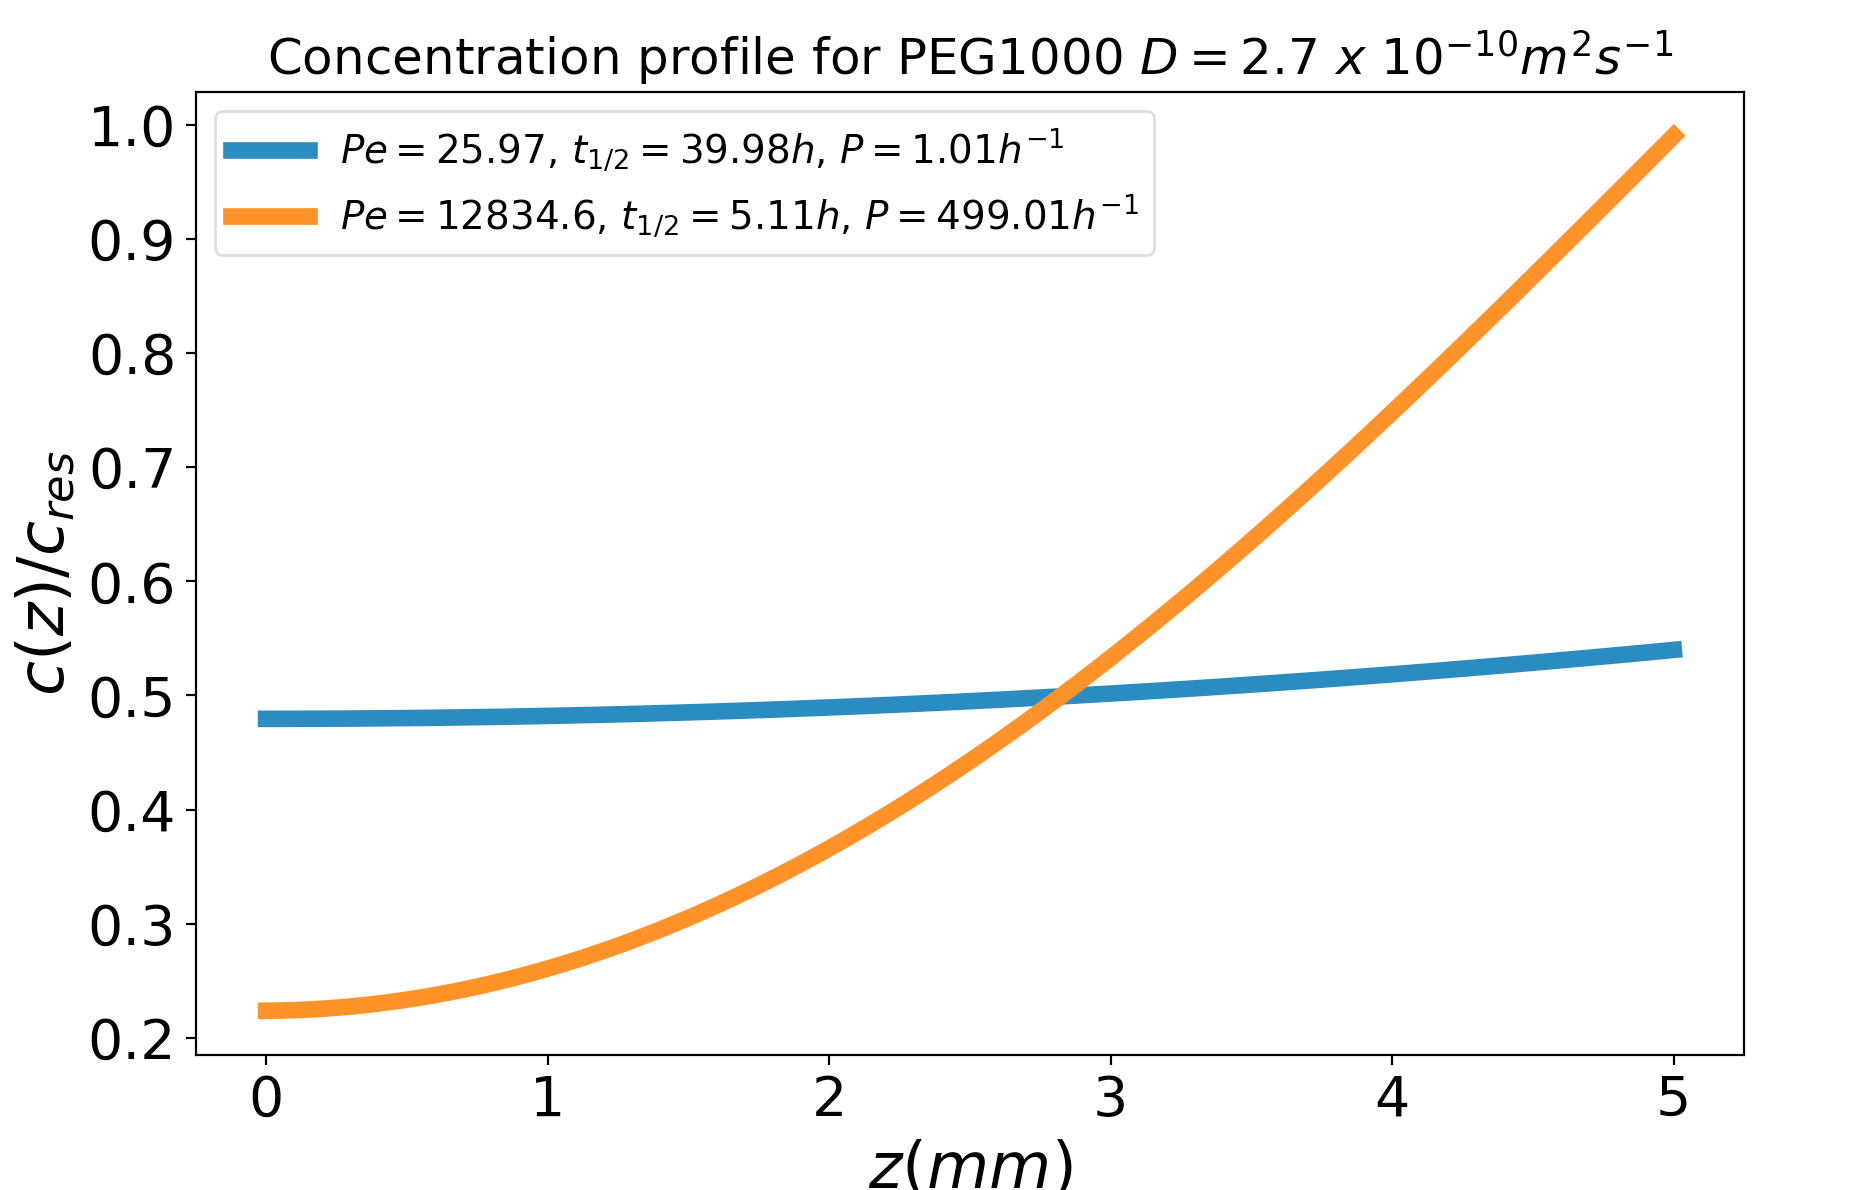
\includegraphics[scale=0.25]{figures/conc_prof_diff_PEG1000_new_2.png}
          \caption{Concentration profile for PEG 1000 for diffusion coefficient 
          $D = 2.7 \times 10^{-10} m^2/s^{-1}$ \label{conc_prof_PEG1000}}
      \end{center} 
    \end{figure}
    \noindent 
    This argument is clearer in Figures \ref{conce_prof_PEG1000_multi} and \ref{conce_prof_NaCl_multi}, where concentration profiles of PEG 1000 and NaCl, respectively, are shown for a large P\'eclet number are shown for 
    multiple times. 

    \begin{figure}[!htb]
      \begin{center}
          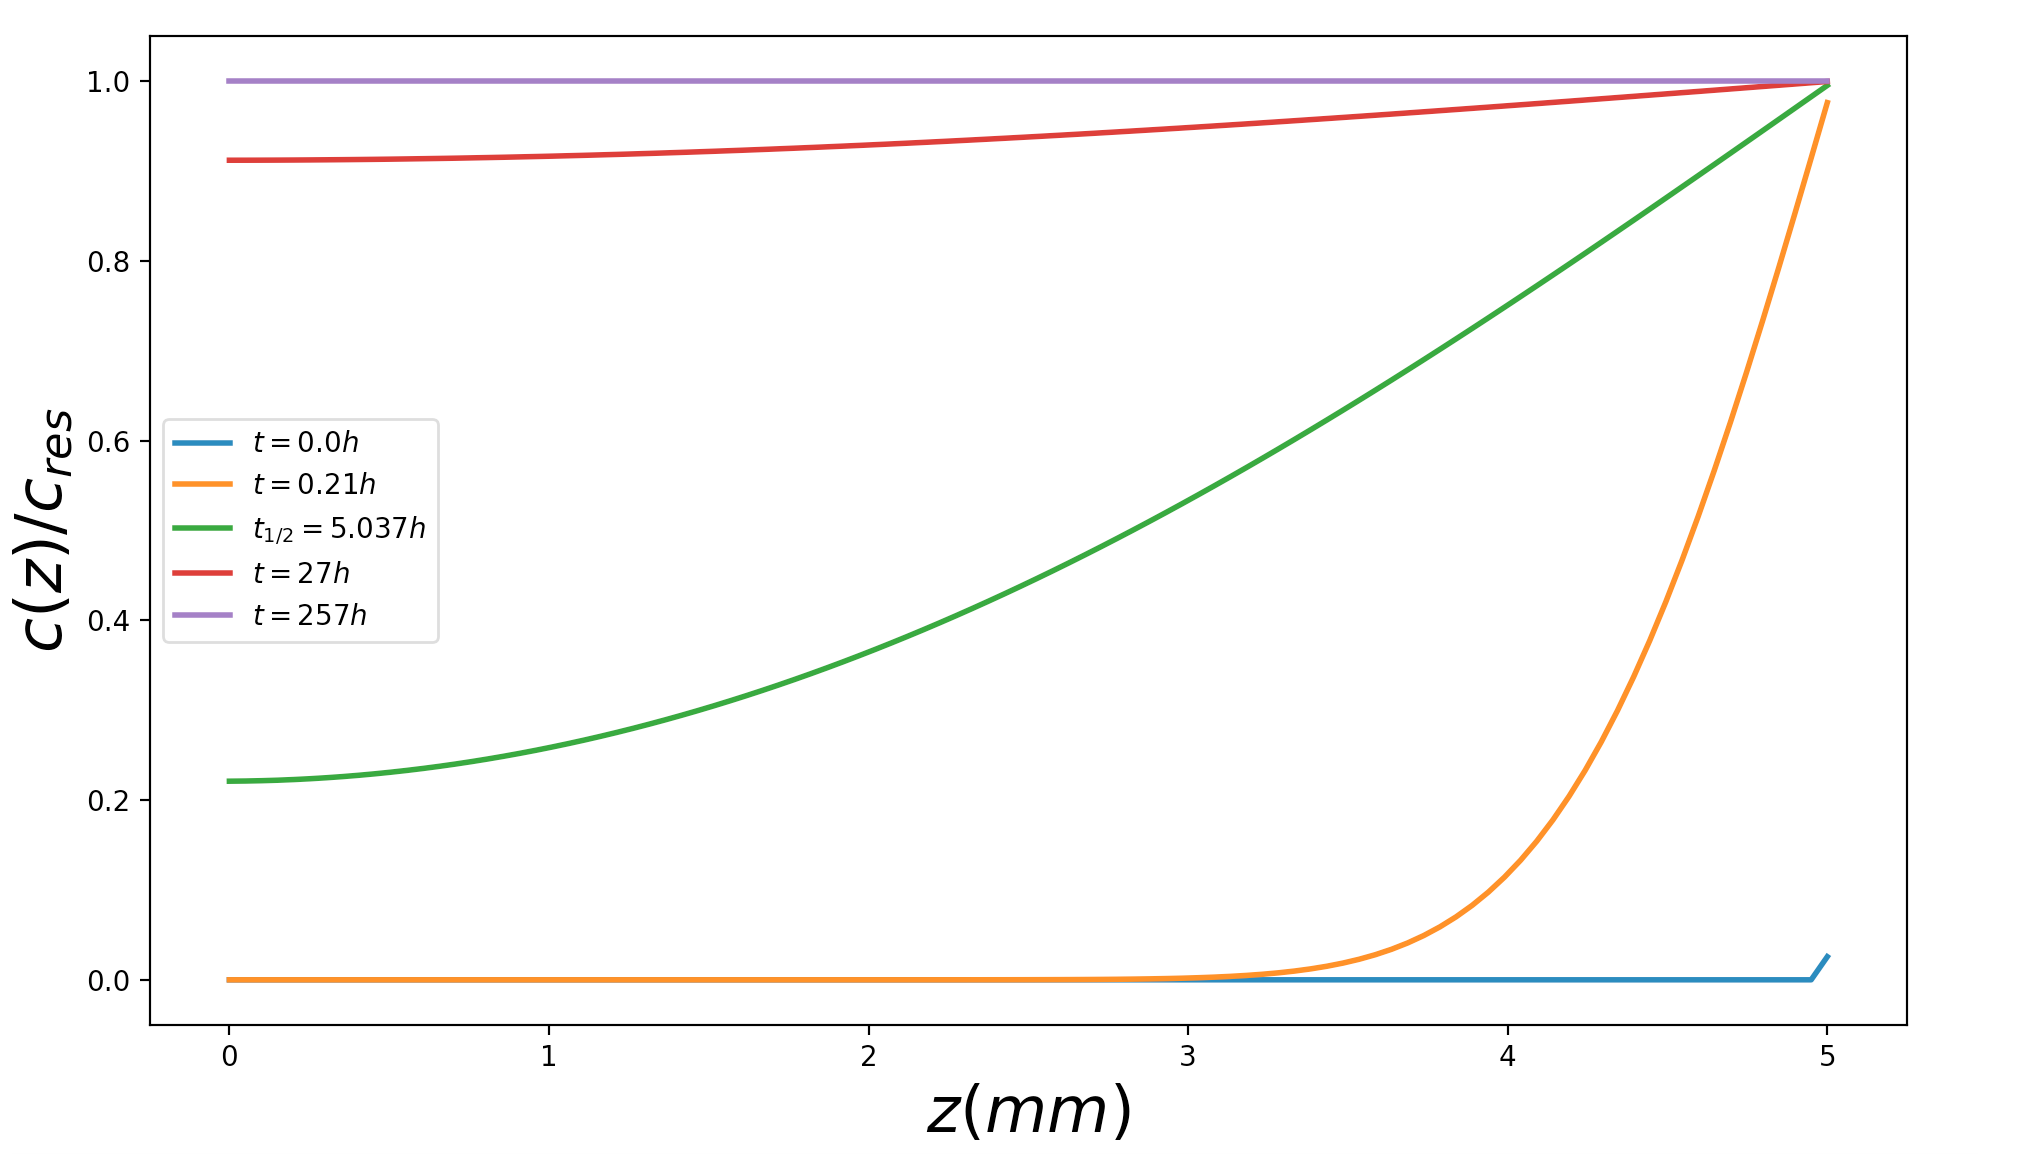
\includegraphics[scale=0.24]{figures/PEG1000_conce_prof.png}
          \caption{Concentration profiles for permeability rate $1{}000 h^{-1}$ and diffusion coeffient of $D = 2.7 \times 10^{-10} m^2/s^{-1}$ \label{conce_prof_PEG1000_multi}}  
      \end{center} 
    \end{figure}
    \noindent 

    \begin{figure}[!htb]
      \begin{center}
          \includegraphics[scale=0.25]{figures/SALT_thalf.png}
           \caption{Concentration profile for PEG 1000 for diffusion coefficient 
          $D = 16 \times 10^{-10} m^2/s^{-1}$ \label{conc_prof_NaCl}}
      \end{center} 
    \end{figure}{}

    \begin{figure}[!htb]
      \begin{center}
          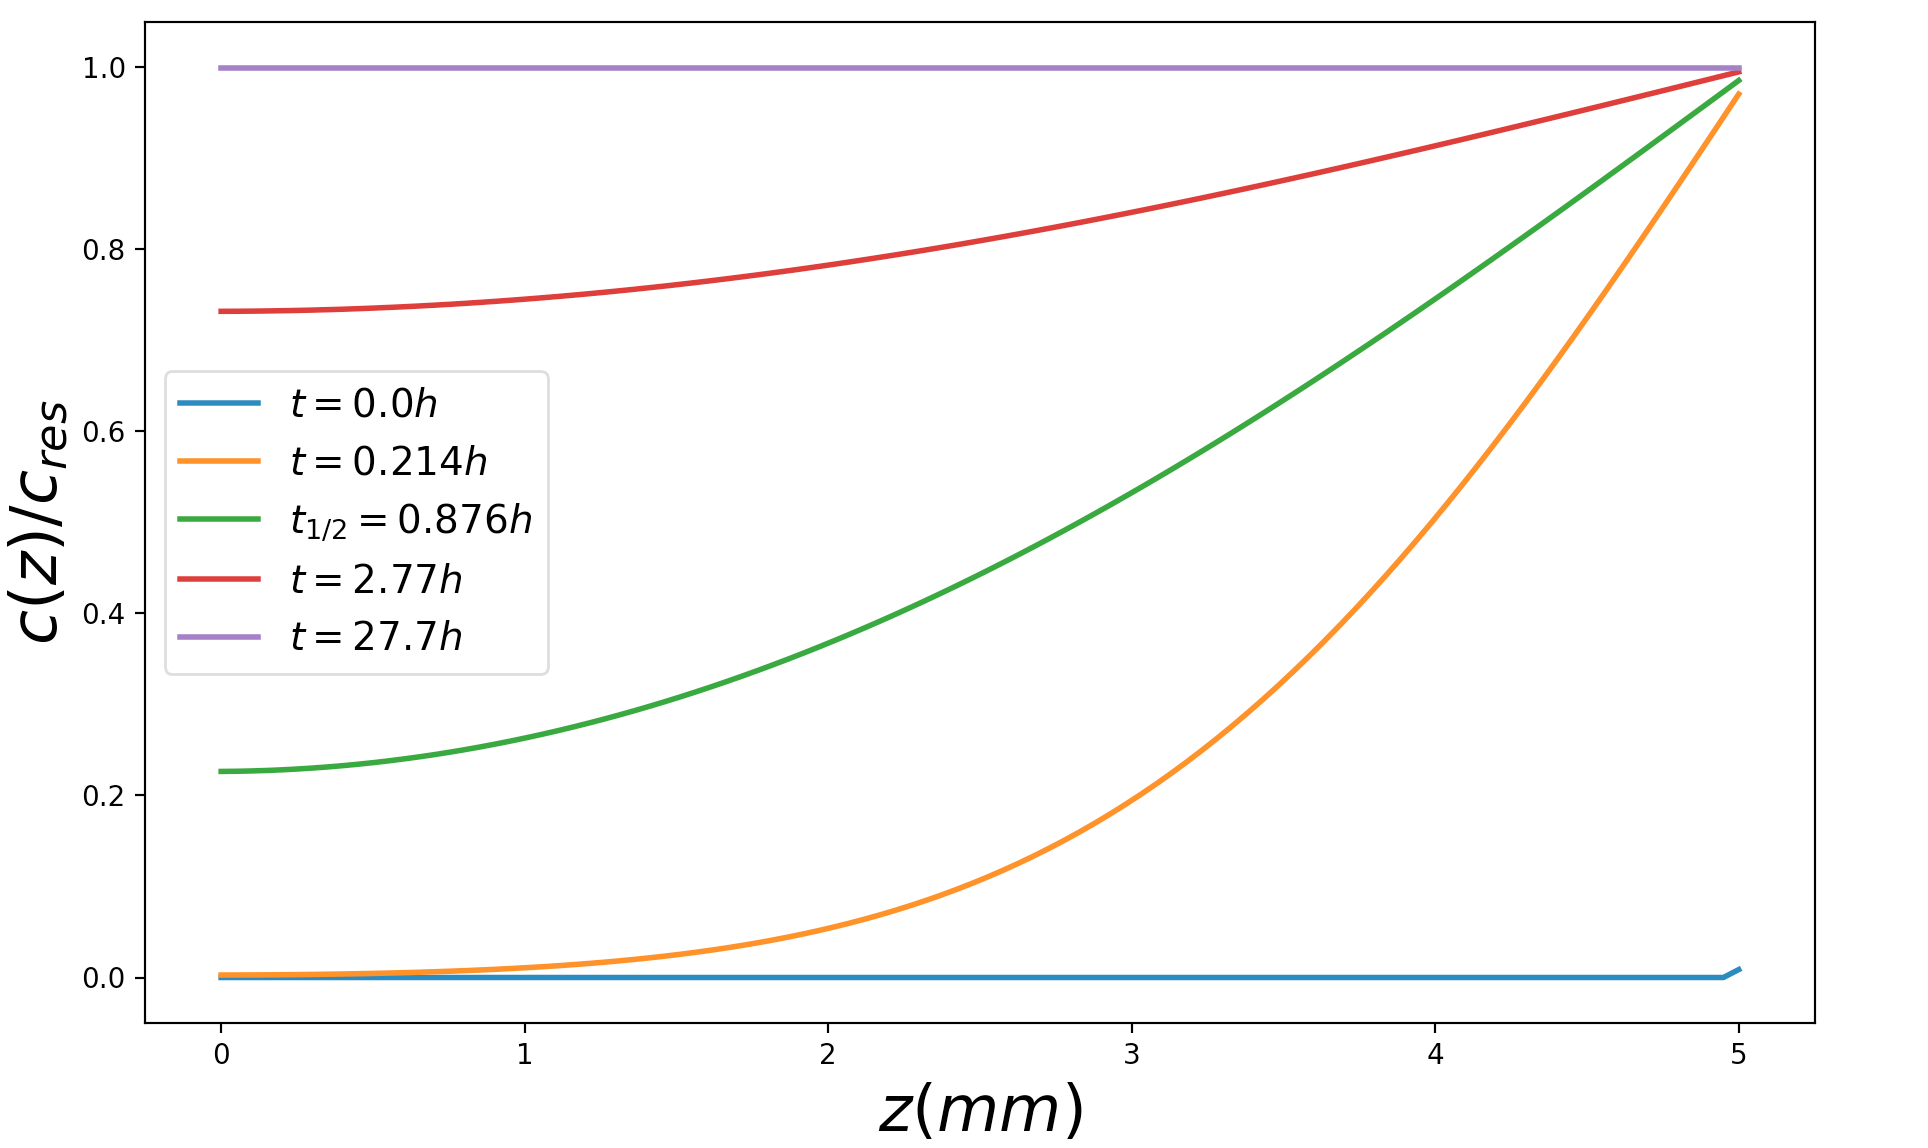
\includegraphics[scale=0.25]{figures/SALT_conc_profiles.png}
          \caption{Concentration profiles for permeability rate $1{}000 h^{-1}$ and diffusion coeffient of $D = 2.7 \times 10^{-10} m^2/s^{-1}$ \label{conce_prof_NaCl_multi}}  
      \end{center} 
    \end{figure}

\subsection*{Error Analysis}

In our analysis, we use the bootstrap method to evaluate the uncertainty of the experimental data. This will give us an estimation of whether or not our model simulates the experimental results satisfactory. The bootstrap is a computational resampling technique for finding standard errors and confidence intervals, with the only input being a set of data. In
practice, the method mimics the process of randomly sampling from an assumed infinite population. Figures \ref{fig_PEG100_CI} and \ref{fig_NACL_CI} shows the confident intervals
for PEG 1000 and NaCl, respectively, for different set of data. The blue curve corresponds to
the results we obtained from the diffusion model. It is shown that for both systems, our model is able to simulate the half-escape values inside the bounds of the statistical error. 


\begin{figure}[!htb]
  \begin{center}
      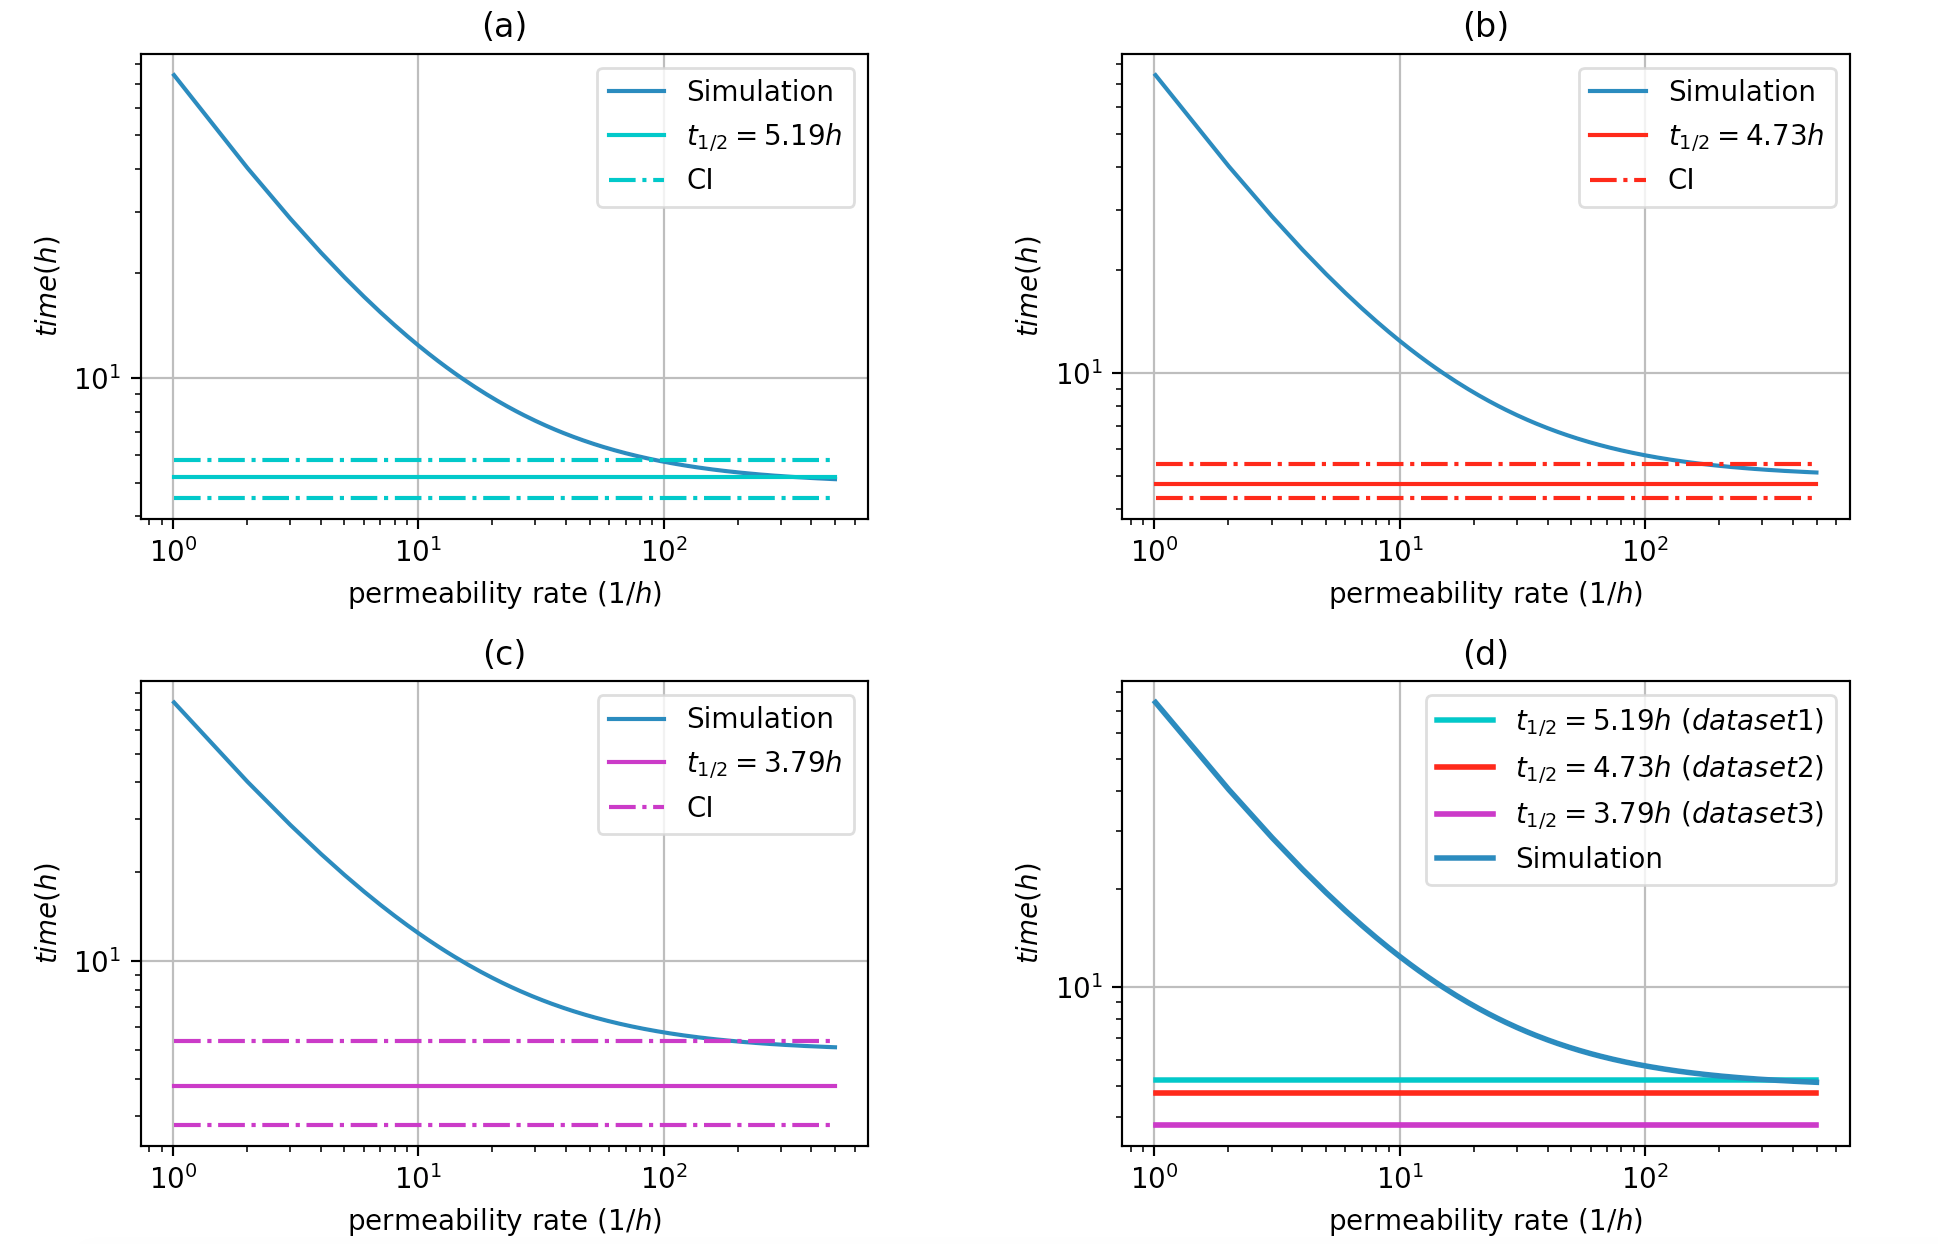
\includegraphics[scale=0.25]{figures/PEG1000_CI.png}
      \caption{\label{fig_PEG100_CI}}  
  \end{center} 
\end{figure}



\begin{figure}[!htb]
  \begin{center}
      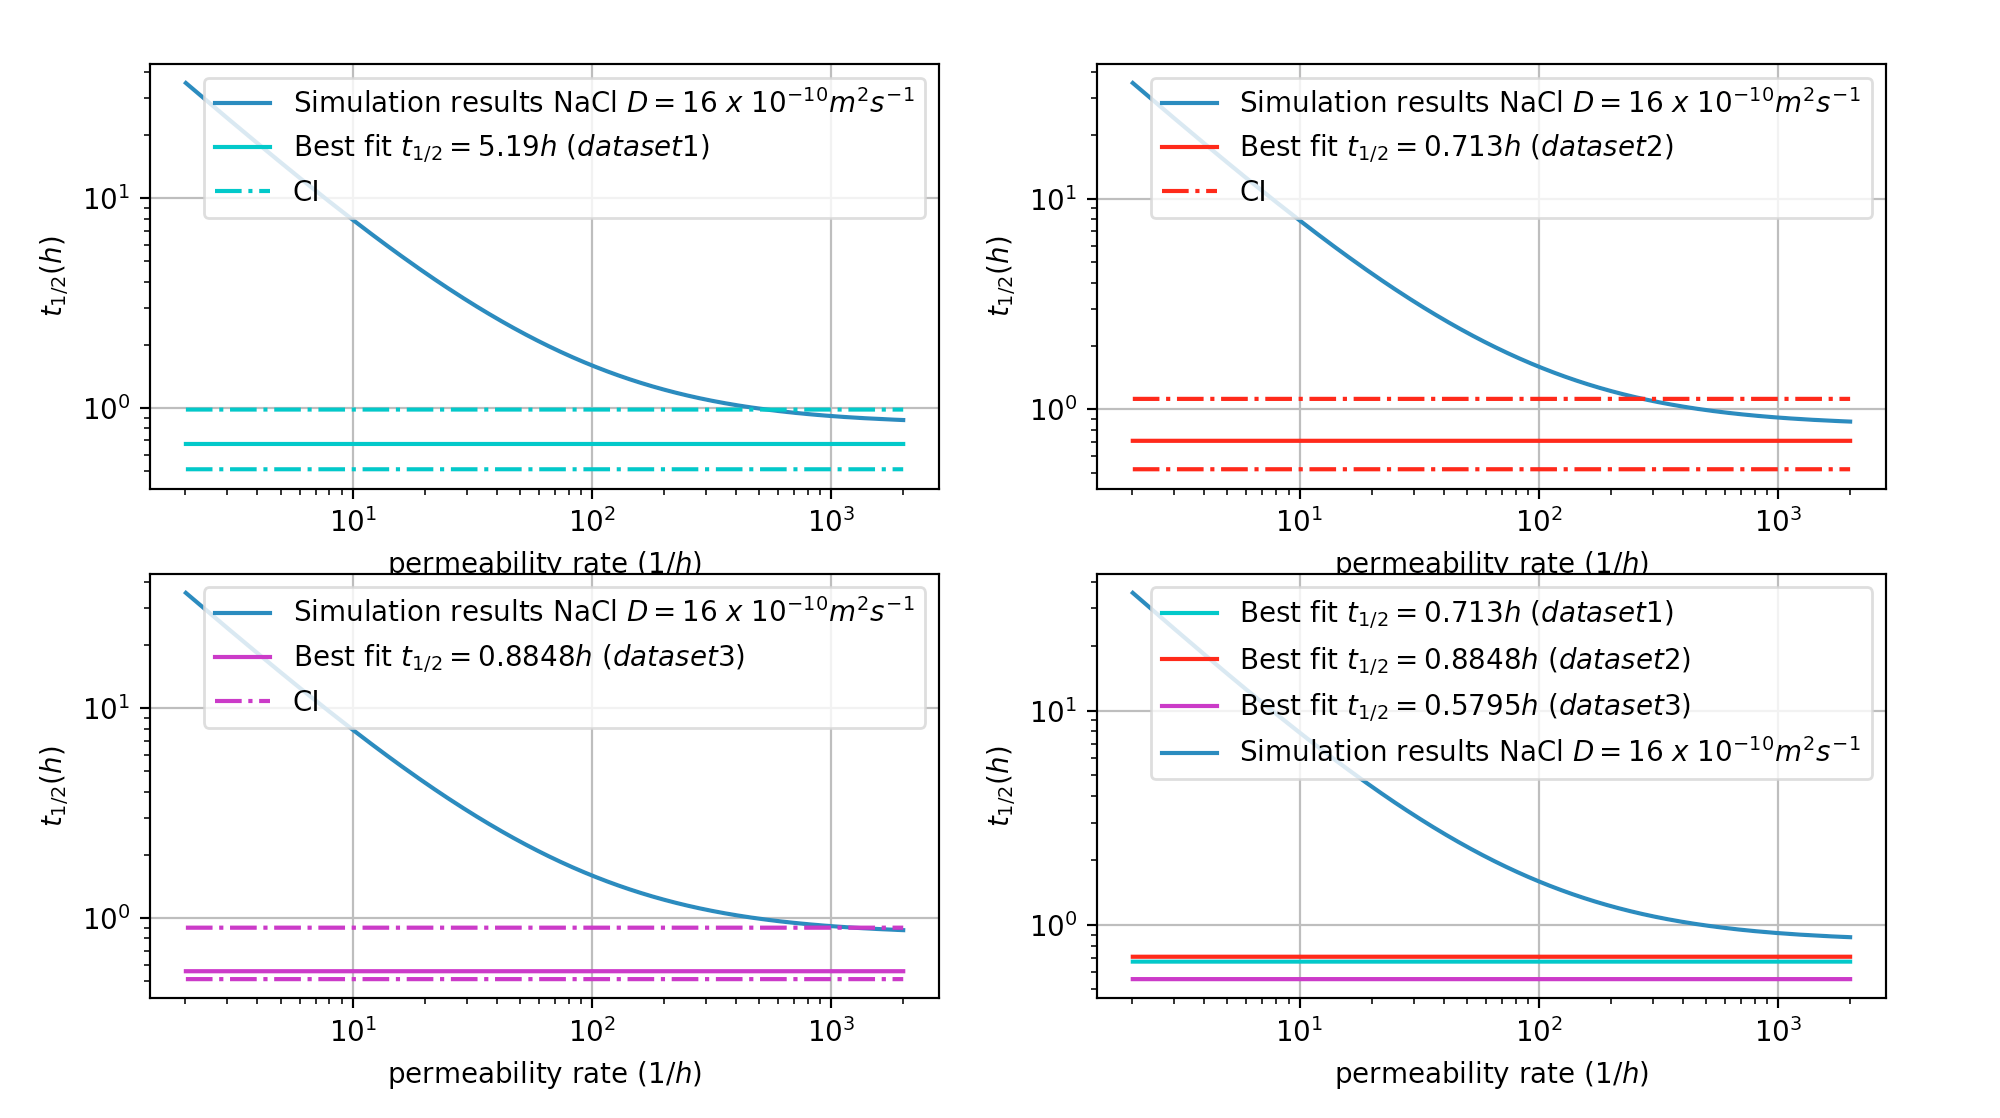
\includegraphics[scale=0.25]{figures/SALT_CI.png}
      \caption{\label{fig_NACL_CI}}
  \end{center} 
\end{figure}


% We can see that for large permeability rate values, the model reaches the $t_{1/2}$ values that 
% we get from the experimental data. This is an indication that the systems are controlled by the 
% permeability, i.e. the time PEG needs to cross across the membrane. 

% Next, we present a figure of concentration profiles, for large permeability values, but for different
% times. 

% \begin{figure}[!htb]
%   \begin{center}
%       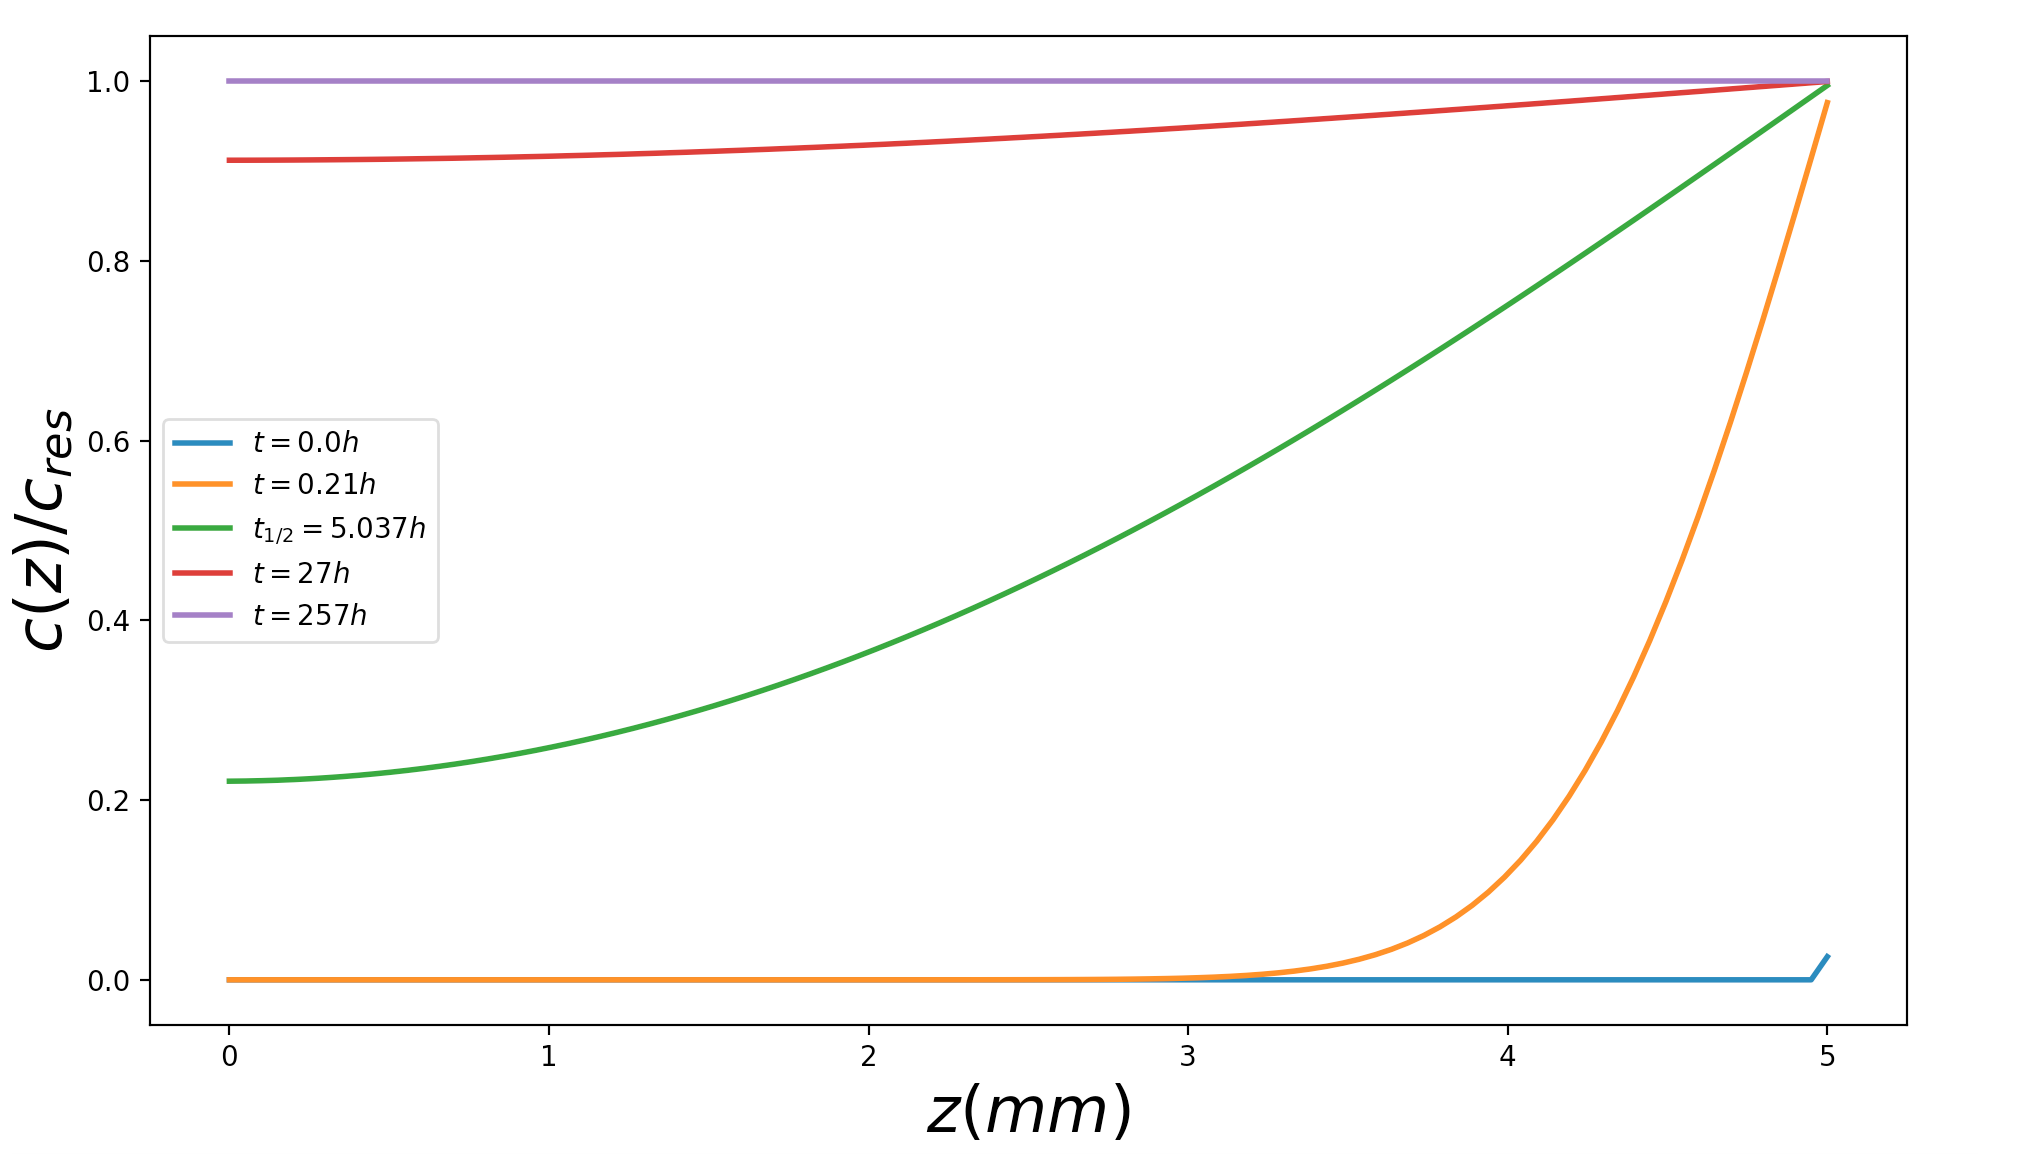
\includegraphics[scale=0.24]{figures/PEG1000_conce_prof.png}
%       \caption{Concentration profiles for permeability rate $1{}000 h^{-1}$ and diffusion coeffient of $D = 2.7 \times 10^{-10} m^2/s^{-1}$}  
%   \end{center} 
% \end{figure}
% \noindent 
% We can see the changes in of the concentration with time and the different gradients.

% We also contacted an error analysis in the data in order to extract confident intervals for the values of $t_{1/2}$ and subsequently, have a more quantitative idea of the errors.
 
% \newline
% The model is able to simulate the best fit $t_{1/2}$ value quite well, 
% always inside the limits of the acceptance region. 


% \subsection*{NaCl}

% \begin{figure}[!htb]
%   \begin{center}
%       \includegraphics[scale=0.25]{fgures/SALT_thalf.png}
%       % \caption{.}  
%   \end{center} 
% \end{figure}{}

% \begin{figure}[!htb]
%   \begin{center}
%       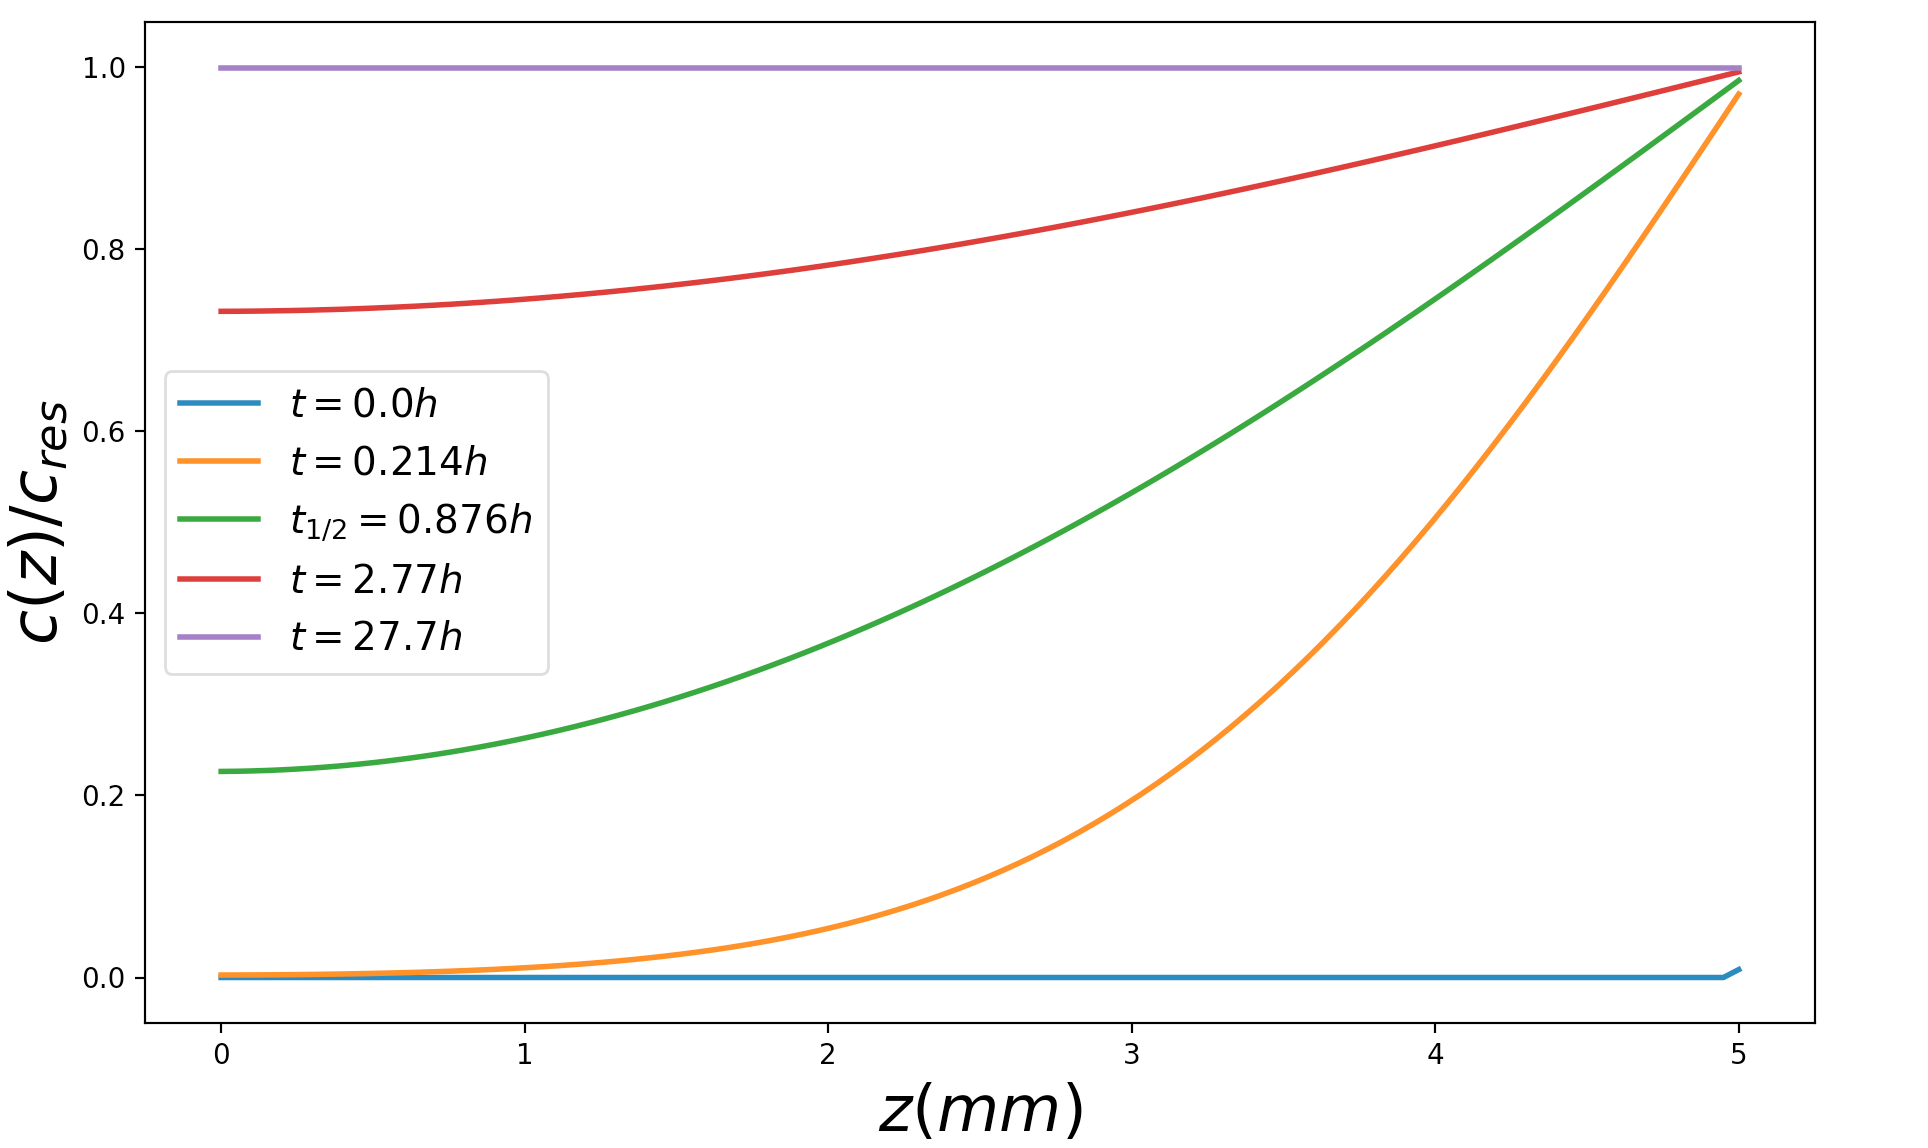
\includegraphics[scale=0.25]{figures/SALT_conc_profiles.png}
%       % \caption{.}  
%   \end{center} 
% \end{figure}


\newpage


\section{Discussion}
kdfjoijnc nsdkfu nsd ncalwi vnsi 


\medskip
\bibliographystyle{unsrt}
\bibliography{ref-paper.bib}

 





\end{document}
